
\section{Basics of Architecture}

Before starting to consider some \verb|C/C++| CUDA code examples, we will look into some architecture of the GPU. 
Indeed, one of the differences between CUDA (or GPU) and usual (sequential) programming \footnote{In our understanding, the
\textit{usual} programming is the code we write in C, Java, Python, etc... to run it on the CPU. It has mostly sequential instructions}, 
is that one must take into account
the architecture of the GPU, even when writing some simple code. The GPU has a multithread architecture by default. 
So when the programmer is partitioning the parallel tasks, he must make sure that there are no redundant
operations, and think about the way the cores will execute these tasks. If this partitioning takes into consideration all necessary aspects of the architecture and memory, it is possible to archive significant performance improvements.


The main difference between the CPU and the GPU is that the GPU has, in a way, lots of smaller CPUs in it, which 
are much less powerful than the actual CPU (\autoref{cpuvsgpu}).
\cite{tuomanen2018hands}

\begin{figure}
   \centering
   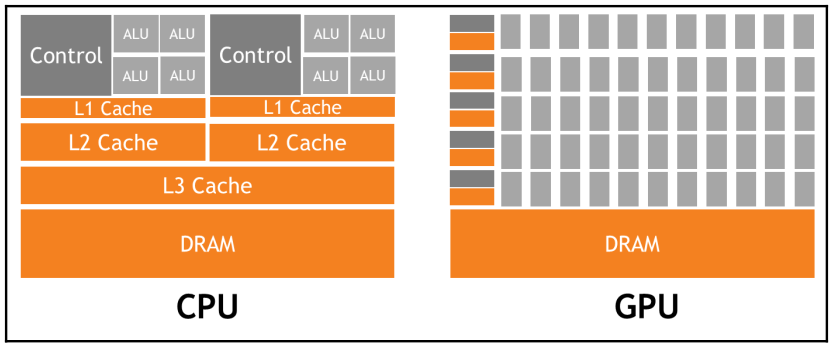
\includegraphics[scale=0.4]{pngs/cpuvsgpu.png}
   \caption{The schematic difference in architecture between the CPU and the GPU. Without going into details 
   (\sout{as mentioned in the disclaimer, the author has not studied it in full depth}), one can see that 
   the GPU has many smaller ALUs. They are less powerful than those of the CPU and don't stand a chance in 
    a theoretical \textit{1v1 battle}, but may do enough \textit{damage}, when working together. Figure from \cite{tuomanen2018hands}.}
   \label{cpuvsgpu}
\end{figure}

\subsection{Execution abstraction}
As you might have noticed, the GPU is by definition a multi-threaded device. This means, it is suitable for the so-called 
SIMT or SIMD (remember the bus and car analogy).


From the hardware viewpoint, we are distinguishing the \textbf{Device (GPU)} itself, the \textbf{Streaming Multiprocessors (SMs)}
, and the \textbf{CUDA cores}. These are physical entities, having a certain structure and features. 
The goal is not to give a detailed description of the GPU architecture, but rather to provide the 
idea of the CUDA mapping between the hardware and software world. While launching a kernel on the device, 
every mentioned part will be assigned a certain role and will treat the software abstractions accordingly.

Us, programmers, we are writing software and operating with software abstractions. However, we still need to know 
how are these abstractions mapped into the \textit{hardware world}.

\vspace{-15pt}
\paragraph{\underline{Threads}} are fundamental units of any GPU program. It is the most primitive \textit{executor} of a function 
launched on the GPU. Threads (from the software side) are executed on the \textbf{CUDA cores} (the hardware side of the program).

\vspace{-15pt}
\paragraph{\underline{Blocks}} \label{blocks} are grouping entities that enclose threads. When a function is asked to run on the GPU, the 
blocks, which \textit{contain} threads are delegated to the corresponding \textbf{Streaming Multiprocessor} or \textbf{SM}.
So by now, we get that 

\begin{quote}
   \centering
   Block of threads $\xrightarrow[]{\text{are transmitted to}}$ SM \newline
   Threads in the block $\xrightarrow[]{\text{are executed on}}$ Cores 
\end{quote} 

So we get that the SMs are partitioning the execution of threads on the Cores at runtime. For example, suppose we have 
launched 8 blocks of let's say 32 threads each. Suppose our GPU has 2 SMs. Then, as mentioned above, 
the blocks are divided and delegated to SMs. Thus for a GPU with 2 SMs, each SM will contain 
$\nicefrac{8\text{blocks}}{2\text{SMs}} = 4 \text{blocks}$, but if our GPU has 4 SMs, 
each SM will contain $\nicefrac{8\text{blocks}}{4\text{threads}} = 2 \text{blocks}$.

Note that from the programmer's viewpoint, the threads are strictly partitioned into blocks. 
From the hardware's viewpoint, however, it is not said, that threads \textit{are physically divided into blocks}. 
This is the exact reason, we are discussing \textit{two worlds} and their mappings/abstractions.

\vspace{-15pt}
\paragraph{\underline{Grid}} is the top-level abstraction layer from the software's perspective. The grid
is the grouping entity that encapsulates blocks. We are thus considering that we are launching 
the grid on the \textbf{device}.
\vspace{-15pt}
\begin{quote}
   \centering
    (Device$\xrightarrow[]{contains}$)Grid $\xrightarrow[]{\text{contains}}$ Blocks $\xrightarrow[]{\text{constains}}$ Threads
\end{quote}

\begin{wrapfigure}{l}{0.5\textwidth}
   \begin{center}
      \vspace{-35pt}
      \centering
       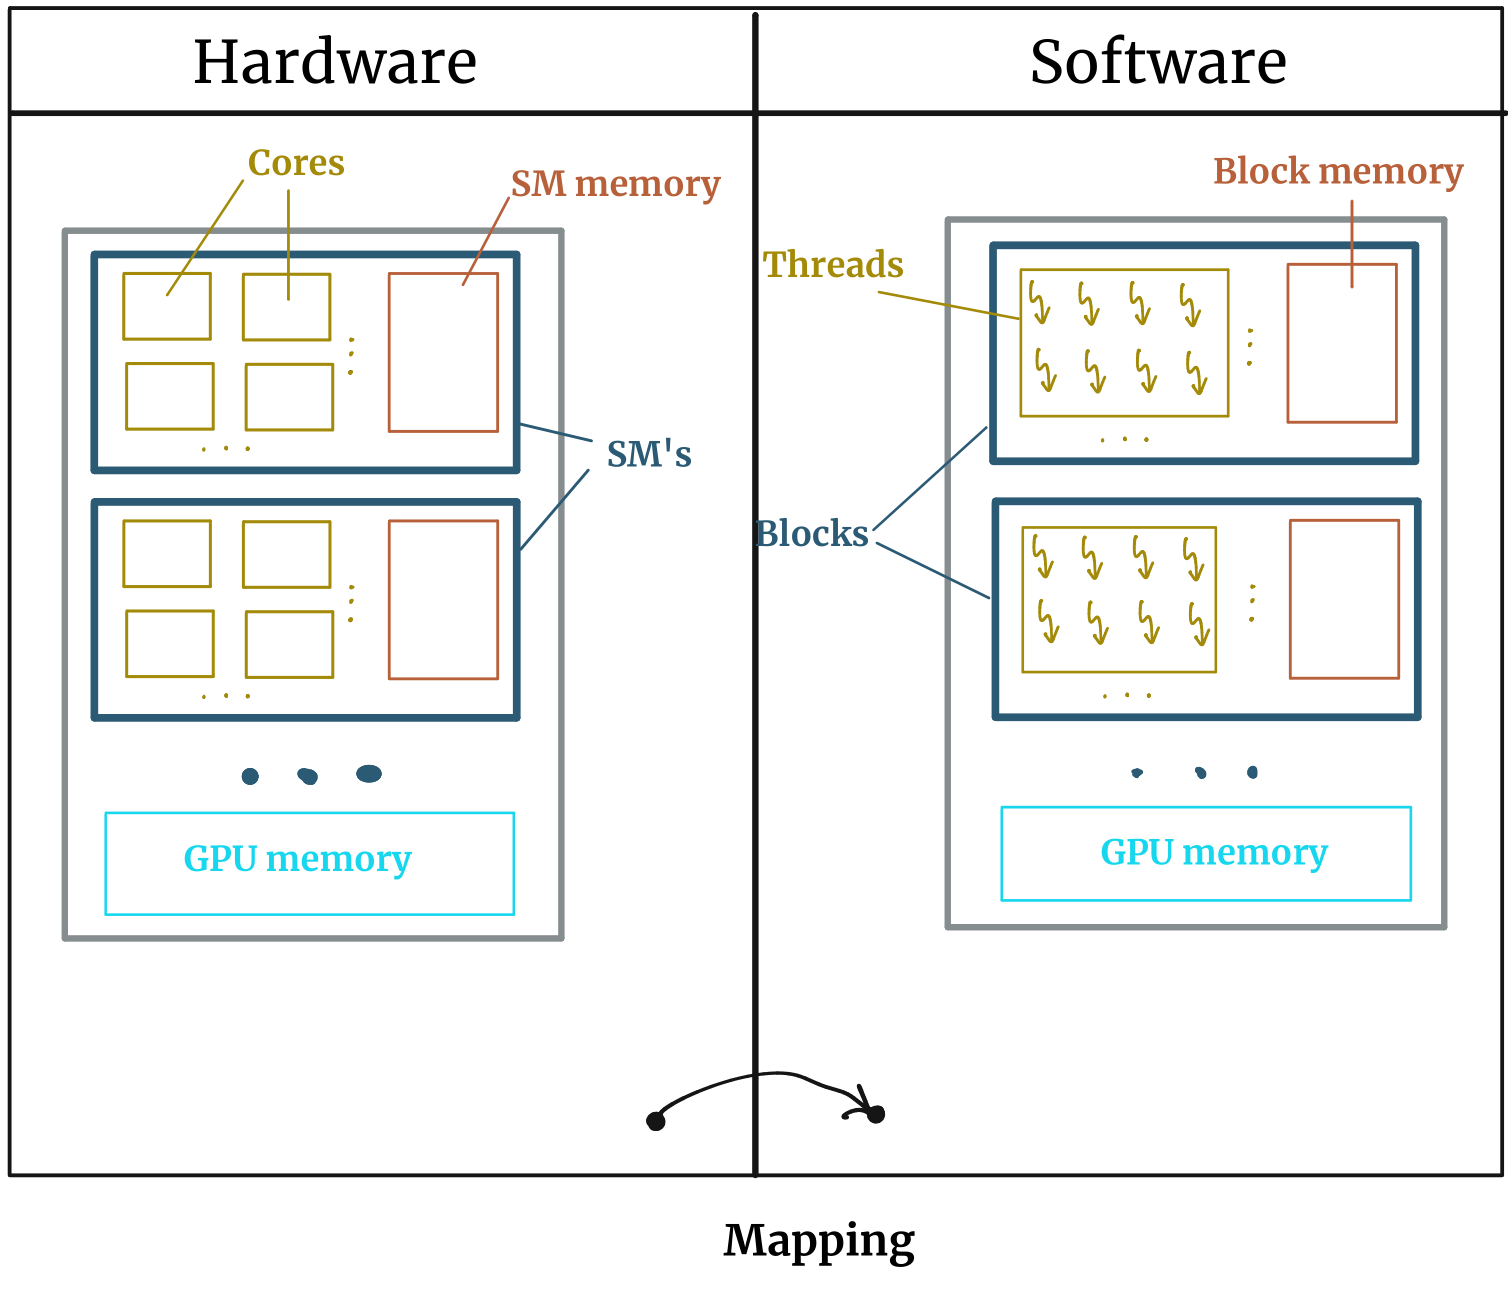
\includegraphics[width=0.4\textwidth]{pngs/hard_soft.png}
    \end{center}
      \vspace{-20pt}
   \caption{Hardware-software abstraction}
   \label{abstraction}
\end{wrapfigure}

\vspace{-18pt}
\paragraph{The mapping abstraction} So to recap the mentioned notions, consider the 
sketch of the hardware/software mapping.

The abstraction between the hardware and the software side of CUDA is shown in \autoref{abstraction}. Once the function 
is provided, the programmer should think of the execution pipeline through threads, blocks, and the grid.

\clearpage
\newpage
\subsection{Parallel execution and warps}
\label{warps}
We briefly saw the anatomy and the terminology of some underlying elements of the CUDA kernel execution.
Conceptually, the threads, to whom a kernel was assigned execute in parallel and are grouped into thread blocks.
Thread blocks run concurrently with each other grouped into a grid. It is important to note (see \autoref{blocks}) that 
the SMs will \textit{automatically} assign the block's execution based on the GPU resources. One may say that 
\textsl{
there is no promise on the block's concurrent execution.
}\cite{tuomanen2018hands}. So we do not know the order in which the blocks will be run.


However, there is a notion, that more or less guarantees the order of the execution of threads. 
\textbf{The Streaming Multiprocessor
treats threads in groups of 32, which are called \underline{warps}}. Think of the warps as a way to handle 
the threads, rather than 
a way of grouping (as the blocks of threads) \footnote{In the AMD terminology, a warp is reffered to as the 
\underline{wavefront}. It brings more insight into the nature of warps}.
We will see that the warps are an extremely important concept of GPU development. 
We will see that the execution of kernel by threads is more efficient when we take into account the fact that 
they are grouped by warps.

\subsection{Memory model}
The memory model of the GPU is quite complicated and different from CPUs memory. It has different fields of memory that have different characteristics-
latency of access, write/read modes, size, scope (to whom it is visible), etc... In the CPU memory, large regions are filled with different level caches. They have similar characteristics. At least, CPU caches are not as different from each other, as the GPU memory types.
First let's take a look into \textbf{general}
notions concerning the memory model.
\vspace{-15pt}
\paragraph{Coalesced vs uncoalesced memory access.} 

\begin{wrapfigure}{l}{0.6\textwidth}
   %\begin{center}
      \vspace{-10pt}
      \centering
      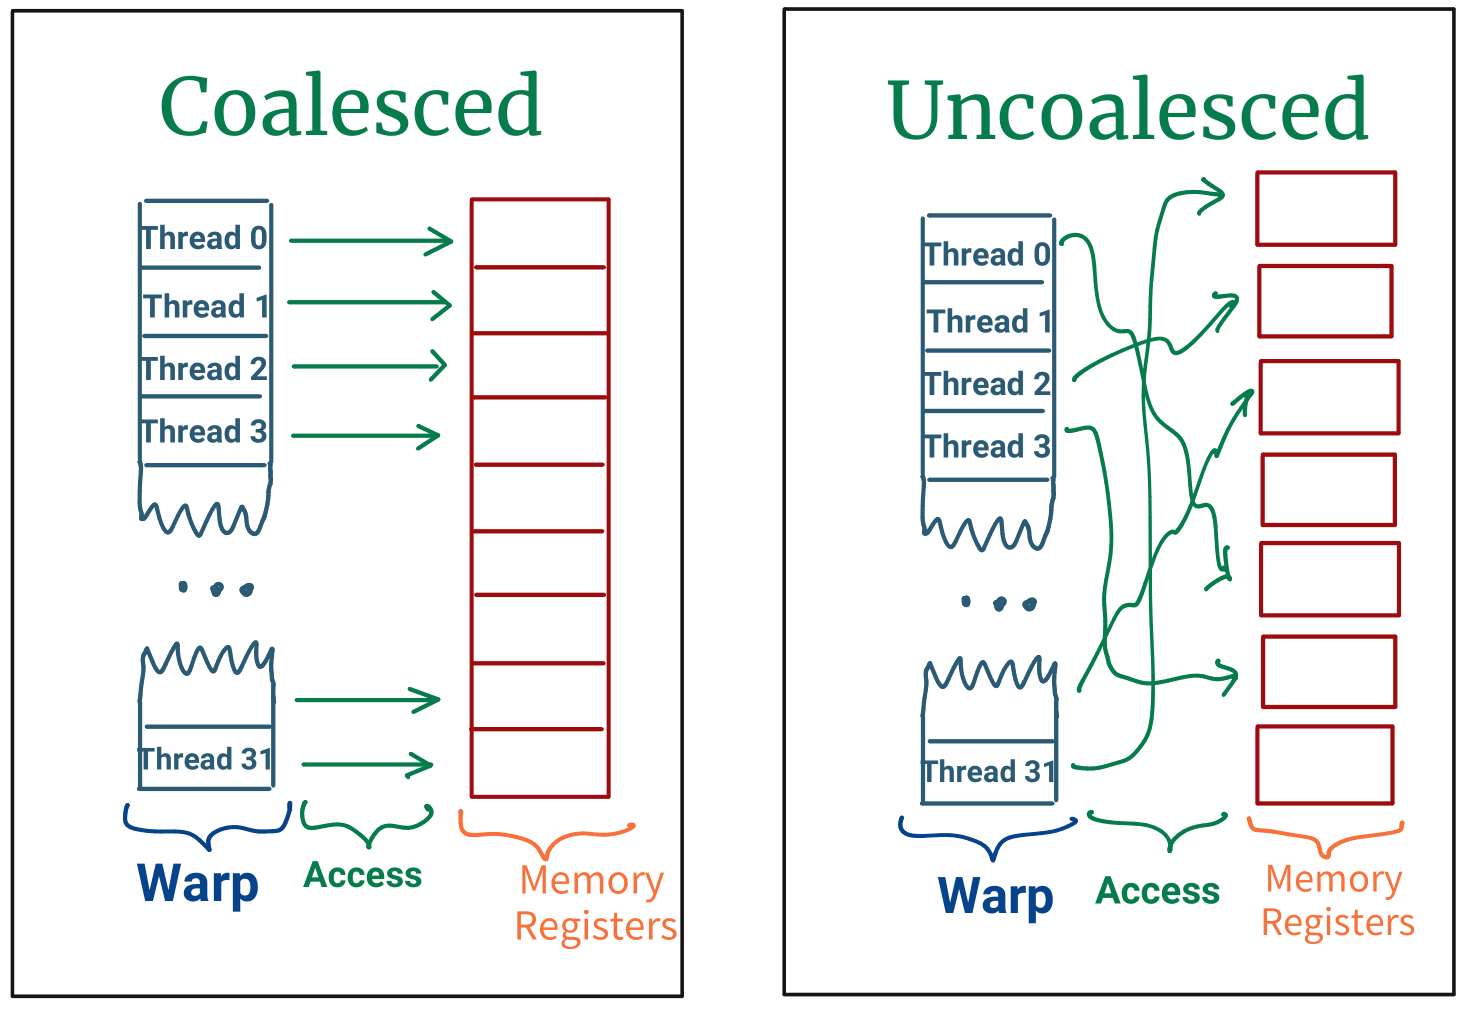
\includegraphics[height=5cm]{pngs/coalesced.png}
    %\end{center}
   \caption{Memory access optimization mechanism.}
   \label{coalesced}
\end{wrapfigure}

Imagine a certain number of warps are scheduled by the SM. Let's say 2 blocks of 128 threads, which gives 
$2\text{blocks}\cdot\nicefrac{128\text{thr.}}{32} = 8 \text{warps}$. These warps fetch some data 
from a certain place in the memory of the GPU. We know that the warp is something very grouped. 
Therefore it would be \textit{nice} them to access adjacent memory addresses. This notion 
may seem quite confusing in the beginning, but let's see how Nvidia is describing it\cite{center}:

\vspace{-10pt}
\begin{quote}
   \textsl{Global memory instructions support reading or writing words \footnote{Words can be data type of a certain size.} 
   of size equal to 1, 2, 4, 8, or 16 bytes. 
   Any access (via a variable or a pointer) to data residing in global memory compiles to a single global memory 
   instruction \textbf{if and only if} the size of the data type is 1, 2, 4, 8, or 16 bytes and the data is naturally aligned 
   (i.e., its address is a multiple of that size). If this size and alignment requirement is not fulfilled, the access 
   compiles to multiple instructions with interleaved access patterns that prevent these instructions from fully coalescing.}
\label{coalescedquote}
\end{quote}
Do not pay attention to the notion of \textbf{global} memory (we will discuss it soon).
Try to read the Nvidia's standard above again by looking at the coalesced scheme (\autoref{coalesced})
to fully understand the mechanism. One may notice that this notion is one of the most crucial in the performance of the code.
Indeed, when writing the kernel, one must keep in mind this aspect and try to ensure (\sout{when possible}) 
a coalesced memory access.

\vspace{-15pt}
\paragraph{\underline{The Global memory}} of the GPU is the largest memory in terms of size, and yet with the greatest latency.
As we've discussed, the kernels are launched \textbf{from} a host (a CPU). It would be wise to be able to share 
resources between the host and the device. For example, send data to the GPU from a usual \verb|C| program
and retrieve it back in a processed form, otherwise, the GPGPU programming does not make sense. 
This is exactly the purpose of global memory. The global memory, as the 
name suggests, is \textsl{global}, i.e. it is \textbf{visible to all threads from all blocks}, and even to the CPU. As we will see in practice,
the usual workflow of the program is to copy the data from the global memory to some other (which is discussed below), 
which is faster \footnote{You may think of it as the {\fontfamily{pcr}\selectfont malloc()} or {\fontfamily{pcr}\selectfont calloc()} functions in C
or the keyword {\fontfamily{pcr}\selectfont new} in C++. Indeed, the allocation and the access to those variables is slower than 
declaring on the stack:\newline {\fontfamily{pcr}\selectfont int $^{\ast}$ ptr\_a = new int; } is slower than {\fontfamily{pcr}\selectfont int a = \{\};}}  
to manipulate. In modern GPU architectures, the global memory is cached. However, we should not rely much on it, 
as even the access to the cached parts of memory is extremely slow compared to other types of memory. We will see in examples, that one of key to a performant program is to minimize the access to this 
slow global memory.

\vspace{-15pt}
\paragraph{\underline{The Shared memory}} \label{grocery_store} is much faster than global one but evidently smaller. Another 
crucial difference between global is the scope - the shared memory is \textbf{only seen by threads in the same block}. This provides 
the ability for threads of the same block to share results and temporary calculations, and process the data \textsc{in place}. 
Think of the following situation: a grocery store, where the customers are threads. Every time a person 
wants to cook something at their house, they don't drive to the store to buy every ingredient needed. They rather go there 
once a week, for example, and buy the amount they need. They also make sure, 
that everything can fit in the fridge. Thus 
in this \sout{wonderful} analogy, the fridge is the low-latency shared memory, and the grocery shop - the 
big and unwieldy global resource - global memory.
One sometimes refers to this memory as 
\textsl{cache memory controlled by the programmer}. However, it is important to take note that the reduced 
latency of the shared memory does not guarantee better performance. Indeed, the biggest pitfall for all \sout{of us} beginners 
is the \textit{bank conflicts}\footnote{A small disclaimer: the notion of \textit{bank conflicts} was one of the reasons for these personal 
notes, as it took a very long time, for the author to understand this concept. The reader should not panic if he's missing something. The examples will be discussed later in the practice part. So one 
should, if necessary, come back to this "theoretical" part after going through the examples. \sout{The author wants to apologize 
for the eventual wordiness.}}. 

\vspace{-0.5cm}
\paragraph{Constant memory} is, as its name suggests constant, thus cannot be changed by the threads during 
the runtime. The constant memory is loaded as static at the beginning of the propram. The constant memory can be 
accessed by all threads in all thread blocks. This memory has a separate caching mechanism, thanks to what, it has 
a low latency. It suits for variables, which do not change over time, which must be accessed by all threads, and, which, 
for some reasons can't be stored in registers.

\paragraph{Texture memory} is the most \textit{special} memory in the list. It is organized into physical 
texture blocks on the GPU. The field of application for texture memory are graphical mechanisms. Despite being a huge topic, we will not discuss 
it in detail here. The reason for that is that we want to use the GPU resources not for graphics, but for its general purpose computational capabilities. The texture memory is used to fill polygons/triangles with textures. This memory 
is often mentioned in the context of CUDA and OpenGL interoperability (see \cite{center} section OpenGL Interoperability).

\paragraph{Local registers}
By looking at the scheme of the architecture of the GPU vs the CPU (\autoref{cpuvsgpu}), one may notice the number 
of registers in the GPU vs the CPU. The amount of registers in the GPU
is incompararble with the registers of the CPU. As you might have guessed, a 
register is a memory, with the scope of a thread. The compiler of a CUDA program will try to optimize the number and size of registers. 
It is nevertheless possible, that the amount of memory in registers may fall short. Then the L1 and/or L2 caches will enter the 
play. This is the fastest memory available in the CUDA API, yet the most restrictive.

\paragraph{Bank conflicts.}We already discussed the notion of warps, as an execution entity encapsulating threads. 
One may think of the \underline{banks} as the analogy of warps in memory
 (i.e. warps are located at the \textit{execution level abstraction}, and the 
 banks-at the \textit{memory level abstraction}). 
 Shared memory is organized into \underline{banks}.
One \textit{layer bank} is a sequential field of 32 memory addresses of 4 bits ($32\text{\#addresses}\cdot 4\text{bits}$). 

\begin{quote}
   \textsl{Memory can serve as many simultaneous address as it has banks.} 
\end{quote}
This is a very important property, so let's consider another \sout{illustrative} analogy. Suppose in a national institution, 
each employee 
is assigned a counter, such that a single employee can serve only one client. Suppose you are the host 
(the person, who assigns people to desks)
and you have a large group of people, whose number is the exact number as the number of desks. The wise choice would be to 
partition them between all the counters, right? Wouldn't that be silly to partition ,let's say 3, to one counter, 4 to 
another, etc... such that there are 8 free counters left. At these 8 counters, the employees will simply wait 
for customers, while there are customers, who are waiting in the queue.
The analogy \sout{may} not be the best, but the sketch should do the trick: 

\begin{figure}[H]
   \centering
   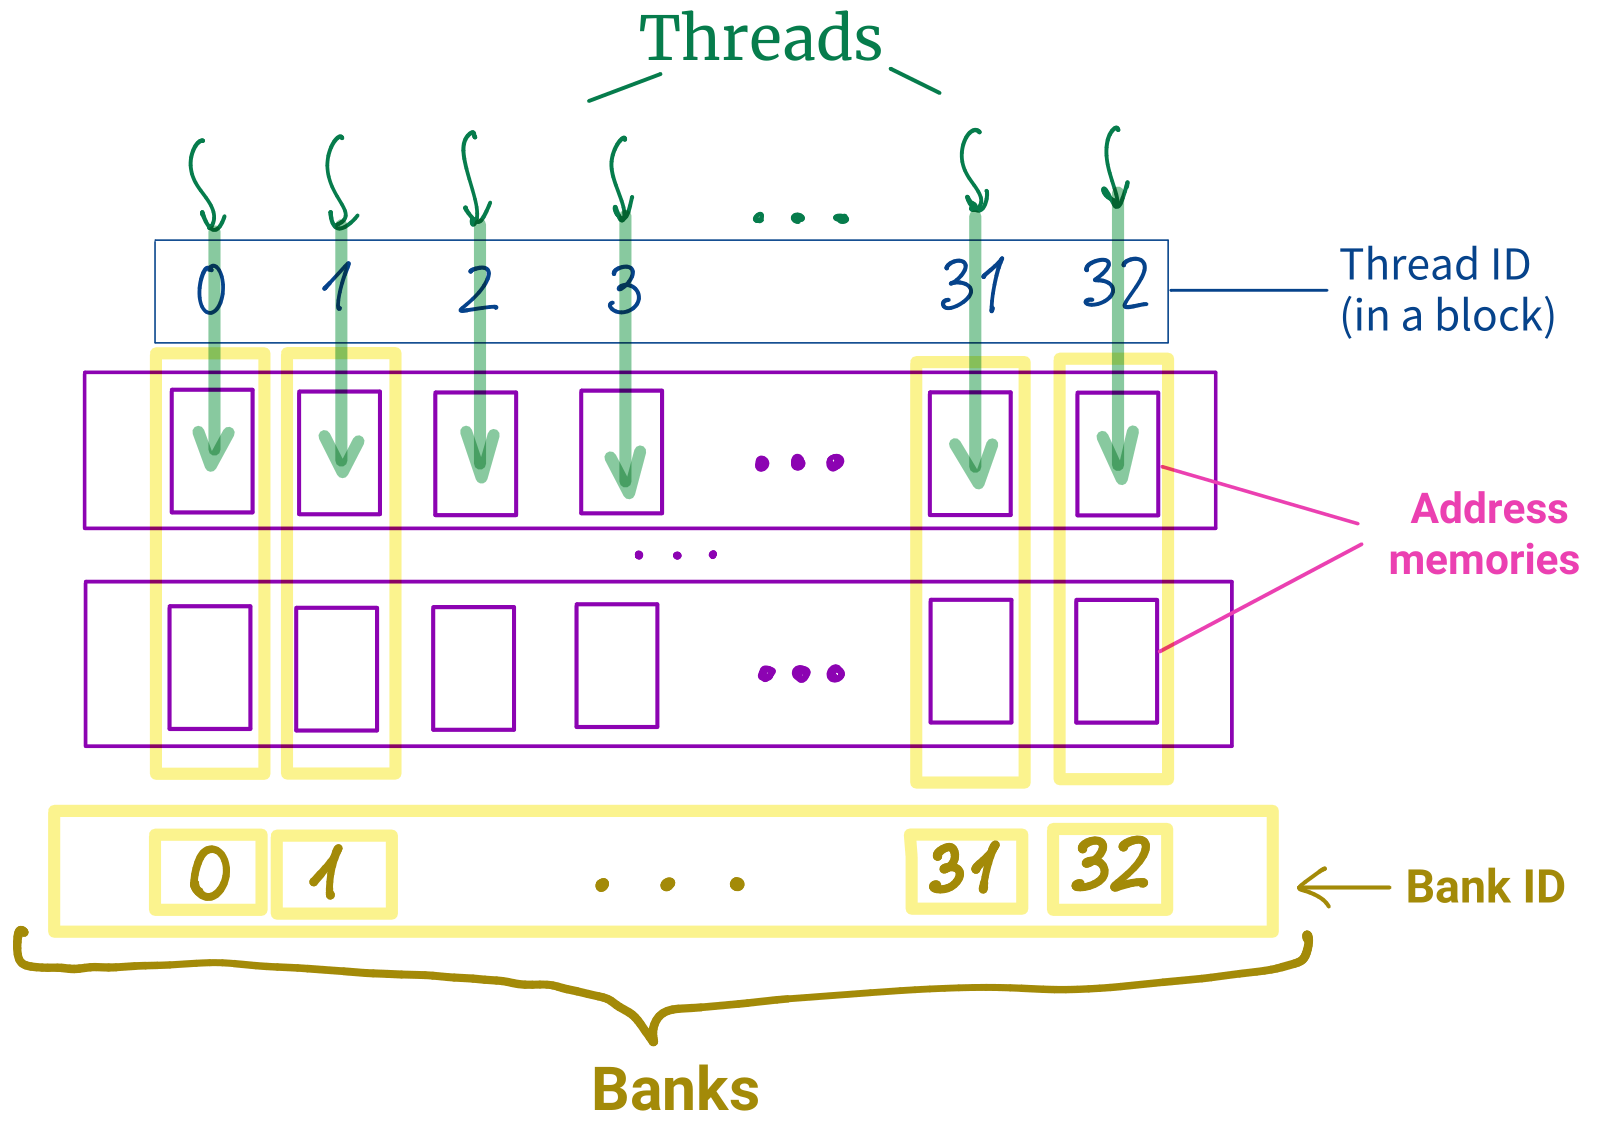
\includegraphics[scale=0.18]{pngs/banks1.png}
   \caption{Memory banks serving threads. Only one thread can access a bank with a certain ID simultaneously. 
   From the analogy, threads are clients, and banks are employees at desks, giving clients memory.}
   \label{banks}

\end{figure}

\subsection{Memory allocation model}
\label{subsection:mem_alloc_model}
By now, we've made the difference between kinds of memory in terms of the scope, i.e, 
\textbf{who} and \textbf{when} can access various kinds of memory. This, of course, somehow impacts the way we're allocating it. 
However, one can classify the memory, in terms of its \textbf{allocation} procedure. There are mainly four ways of memory allocation.

We will see further that a standard
program, which uses GPU resources, follows a certain path/pipeline. 
Roughly that is: 
\begin{enumerate}
\setlength\itemsep{-0.1em}
  \item Resource declaration on the host (using \verb|malloc|) and initialization using \verb|memcpy|.
  \item Memory allocation and initialization on the device.
  \item Memory copying/transfer from the host to device.
  \item Accelerated computation on the GPU and storage of the results from the device
  \item Copy data from the device back to the host.
\end{enumerate}

One of the steps is the allocation of 
memory on the GPU from the host (by calling a certain CUDA function, which will be described later). 
\begin{itemize}
\setlength\itemsep{-0.1em}
   \item Pageable memory
   \item Pinned memory
   \item Mapped memory
   \item Unified memory
\end{itemize}
The difference in terms of the API calls, use cases, and mechanisms, will be explained further \autoref{subsub:mem_mapping}. 



